\chapter{Appendix}
\label{apx:appendix}

\begin{figure}[!htb]
\sbox0{\subcaptionbox{Vertical stress, longitudinal particle displacement\label{sfig:piezo_beam}}{%
        
\includegraphics[scale=0.7]{figures/measurement/piezo/piezo_beam}
        }}% a
    \sbox1{\subcaptionbox{Vertical stress, lateral particle displacement\label{sfig:piezo_plate_top}}{%
        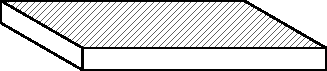
\includegraphics[scale=0.7]{figures/measurement/piezo/piezo_plate_top}
        }}% b
    \sbox2{\subcaptionbox{Vertical stress, lateral particle displacement\label{sfig:piezo_plate_side}}{%
        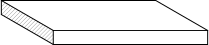
\includegraphics[scale=0.7]{figures/measurement/piezo/piezo_plate_side}
        }}% c
    \sbox3{\subcaptionbox{Lateral stress, lateral particle displacement\label{sfig:piezo_radial_long}}{%
        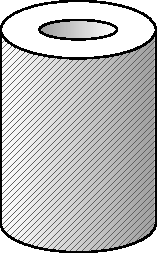
\includegraphics[scale=0.7]{figures/measurement/piezo/piezo_radial_long}
        }}% d
    \sbox4{\subcaptionbox{Radial particle displacement\label{sfig:piezo_radial_flat}}{%
        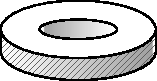
\includegraphics[scale=0.7]{figures/measurement/piezo/piezo_radial_flat}
        }}% e
    \sbox5{\subcaptionbox{Radial particle displacement\label{sfig:piezo_axial_hole_flat}}{%
        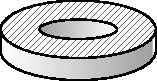
\includegraphics[scale=0.7]{figures/measurement/piezo/piezo_axial_hole_flat}
        }}% f
    \sbox6{\subcaptionbox{Vertical stress, radial particle displacement\label{sfig:piezo_sphere}}{%
        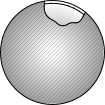
\includegraphics[scale=0.7]{figures/measurement/piezo/piezo_sphere}
        }}% g
    \sbox7{\subcaptionbox{Radial particle displacement\label{sfig:piezo_axial_flat}}{%
        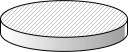
\includegraphics[scale=0.7]{figures/measurement/piezo/piezo_axial_flat}
       }}% h
    \sbox8{\subcaptionbox{Radial particle displacement\label{sfig:piezo_radial_rod}}{%
        
\includegraphics[scale=0.7]{figures/measurement/piezo/piezo_radial_rod}
       }}% i
    \centering
    {%
        \renewcommand{\arraystretch}{4}%
        \setlength{\tabcolsep}{2em}
        \begin{tabular}{ccc}
            \usebox0 & \usebox3 & \usebox6 \\
            \usebox1 & \usebox4 & \usebox7 \\
            \usebox2 & \usebox5 & \usebox8
        \end{tabular}
    }
    \caption[Piezoelectric designs]{Piezoelectric designs, where electrodes are placed on the shaded areas}
    \label{fig:piezo_designs}
\end{figure}

\begin{figure}[!htb]
    \centering
    \includestandalone[scale=0.8]{figures/electronics/ic_flowchart/ic_flowchart}
    \caption[IC packages flowchart]{Flowchart of IC packages}
    \label{fig:ic_flowchart}
\end{figure}
{\scriptsize%
\begin{longtable}{lccc}
\caption[Andromeda Measurements, Prototype Impact Hammer]{Andromeda measurement setup that is excited by the prototype impact hammer. The prototype accelerometer is set to a dynamic range of $\pm$\SI{16}{g} and a \acs{AAF} cut-off of \SI{800}{\hertz}.}\\
\toprule
Label & \makecell{Excitation\\Location} & \makecell{Prototype Sampling\\Rate / \si{\kilo\hertz}} & \makecell{Prototype Recording\\Duration / \si{\second}}\\
\midrule
\endfirsthead
\caption[]{(Continued)}\\
\toprule
Label & \makecell{Excitation\\Location} & \makecell{Prototype Sampling\\Rate / \si{\kilo\hertz}} & \makecell{Prototype Recording\\Duration / \si{\second}}\\
\midrule
\endhead
\midrule
\multicolumn{4}{c}{continued on next page}\\
\bottomrule
\endfoot
%\bottomrule
\endlastfoot
\hline
	HAe001 & A & 1.6 & 3\\ 
	HAe002 & A & 1.6 & 3\\ 
	HAe003 & A & 1.6 & 3\\ 
	HAe004 & A & 1.6 & 3\\ 
	HAe005 & A & 1.6 & 3\\ 
	HAe006 & B & 1.6 & 3\\
	HAe007 & B & 1.6 & 3\\
	HAe008 & B & 1.6 & 3\\
	HAe009 & B & 1.6 & 3\\
	HAe010 & B & 1.6 & 3\\
	HAe011 & C & 1.6 & 3\\
	HAe012 & C & 1.6 & 3\\
	HAe013 & C & 1.6 & 3\\
	HAe014 & C & 1.6 & 3\\
	HAe015 & C & 1.6 & 3\\
	HAe016 & D & 1.6 & 3\\
	HAe017 & D & 1.6 & 3\\
	HAe018 & D & 1.6 & 3\\
	HAe019 & D & 1.6 & 3\\
	HAe020 & D & 1.6 & 3\\
\bottomrule
\label{tab:hae_tests}
\end{longtable}
}

{\scriptsize%
\begin{longtable}{lccccc}
\caption[Andromeda Measurements, Reference Impact Hammer]{Andromeda measurement setup that is excited by the reference impact hammer}\\
\toprule
Label & \makecell{Excitation\\Location} & \makecell{Accelerometer Sampling\\Rate / \si{\kilo\hertz}} & \makecell{Prototype Recording\\Duration / \si{\second}} & \makecell{Accelrometer\\Dynamic Range / \si{g}} & \makecell{Accelerometer\\AAF cut-off / \si{\hertz}}\\
\midrule
\endfirsthead
\caption[]{(Continued)}\\
\toprule
Label & \makecell{Excitation\\Location} & \makecell{Accelerometer Sampling\\Rate / \si{\kilo\hertz}} & \makecell{Prototype Recording\\Duration / \si{\second}} & \makecell{Accelrometer\\Dynamic Range / \si{g}} & \makecell{Accelerometer\\AAF cut-off / \si{\hertz}}\\
\midrule
\endhead
\midrule
\multicolumn{6}{c}{continued on next page}\\
\bottomrule
\endfoot
%\bottomrule
\endlastfoot
\hline
    HAp001 & A & 1.6 & 3 & $\pm$16 & 800\\
	HAp002 & A & 1.6 & 3 & $\pm$16 & 800\\
	HAp003 & A & 1.6 & 3 & $\pm$16 & 800\\
	HAp004 & A & 1.6 & 3 & $\pm$16 & 800\\
	HAp005 & A & 1.6 & 3 & $\pm$16 & 800\\
	HAp006 & B & 1.6 & 3 & $\pm$16 & 800\\
	HAp007 & B & 1.6 & 3 & $\pm$16 & 800\\
	HAp008 & B & 1.6 & 3 & $\pm$16 & 800\\
	HAp009 & B & 1.6 & 3 & $\pm$16 & 800\\
	HAp010 & B & 1.6 & 3 & $\pm$16 & 800\\
	HAp011 & C & 1.6 & 3 & $\pm$16 & 800\\
	HAp012 & C & 1.6 & 3 & $\pm$16 & 800\\
	HAp013 & C & 1.6 & 3 & $\pm$16 & 800\\
	HAp014 & C & 1.6 & 3 & $\pm$16 & 800\\
	HAp015 & C & 1.6 & 3 & $\pm$16 & 800\\
	HAp016 & D & 1.6 & 3 & $\pm$16 & 800\\
	HAp017 & D & 1.6 & 3 & $\pm$16 & 800\\
	HAp018 & D & 1.6 & 3 & $\pm$16 & 800\\
	HAp019 & D & 1.6 & 3 & $\pm$16 & 800\\
	HAp020 & D & 1.6 & 3 & $\pm$16 & 800\\
	HAp001 & A & 0.8 & 3 & $\pm$16 & 400\\
	HAp002 & A & 0.8 & 3 & $\pm$16 & 400\\
	HAp003 & A & 0.8 & 3 & $\pm$16 & 400\\
	HAp004 & A & 0.8 & 3 & $\pm$16 & 400\\
	HAp005 & A & 0.8 & 3 & $\pm$16 & 400\\
	HAp006 & B & 0.8 & 3 & $\pm$16 & 400\\
	HAp007 & B & 0.8 & 3 & $\pm$16 & 400\\
	HAp008 & B & 0.8 & 3 & $\pm$16 & 400\\
	HAp009 & B & 0.8 & 3 & $\pm$16 & 400\\
	HAp010 & B & 0.8 & 3 & $\pm$16 & 400\\
	HAp011 & C & 0.8 & 3 & $\pm$16 & 400\\
	HAp012 & C & 0.8 & 3 & $\pm$16 & 400\\
	HAp013 & C & 0.8 & 3 & $\pm$16 & 400\\
	HAp014 & C & 0.8 & 3 & $\pm$16 & 400\\
	HAp015 & C & 0.8 & 3 & $\pm$16 & 400\\
	HAp016 & D & 0.8 & 3 & $\pm$16 & 400\\
	HAp017 & D & 0.8 & 3 & $\pm$16 & 400\\
	HAp018 & D & 0.8 & 3 & $\pm$16 & 400\\
	HAp019 & D & 0.8 & 3 & $\pm$16 & 400\\
	HAp020 & D & 0.8 & 3 & $\pm$16 & 400\\
	HAp021 & C & 1.6 & 3 & $\pm$4 & 800\\
	HAp022 & C & 1.6 & 3 & $\pm$4 & 800\\
	HAp023 & C & 1.6 & 3 & $\pm$4 & 800\\
	HAp024 & C & 1.6 & 3 & $\pm$4 & 800\\
	HAp025 & C & 1.6 & 3 & $\pm$4 & 800\\
	HAp026 & D & 1.6 & 3 & $\pm$2 & 800\\
	HAp027 & D & 1.6 & 3 & $\pm$2 & 800\\
	HAp028 & D & 1.6 & 3 & $\pm$4 & 800\\
	HAp029 & D & 1.6 & 3 & $\pm$4 & 800\\
	HAp030 & D & 1.6 & 3 & $\pm$4 & 800\\
\bottomrule
\label{tab:hap_tests}
\end{longtable}
}

{\scriptsize%
\begin{longtable}{lccc}
\caption[Hammer-Hammer Test Measurements]{Hammer-hammer test measurements}\\
\toprule
Label & \makecell{Prototype\\tip} & \makecell{Prototype Sampling\\Rate / \si{\kilo\hertz}} & \makecell{Prototype Recording\\Duration / \si{\second}}\\
\midrule
\endfirsthead
\caption[]{(Continued)}\\
\toprule
Label & \makecell{Prototype\\tip} & \makecell{Prototype Sampling\\Rate / \si{\kilo\hertz}} & \makecell{Prototype Recording\\Duration / \si{\second}}\\
\midrule
\endhead
\midrule
\multicolumn{4}{c}{continued on next page}\\
\bottomrule
\endfoot
%\bottomrule
\endlastfoot
\hline
	HH001 & 34CrMo4 & 3 & 4\\
	HH002 & 34CrMo4 & 3 & 4\\
	HH003 & 34CrMo4 & 3 & 4\\
	HH004 & 34CrMo4 & 3 & 4\\
	HH005 & 34CrMo4 & 3 & 4\\
	HH006 & 34CrMo4 & 3 & 4\\
	HH007 & 34CrMo4 & 3 & 4\\
	HH008 & 34CrMo4 & 3 & 4\\
	HH009 & 34CrMo4 & 3 & 4\\
	HH010 & 34CrMo4 & 3 & 4\\
	HH011 & 34CrMo4 & 3 & 3\\
	HH012 & 34CrMo4 & 2 & 3\\
	HH013 & 34CrMo4 & 2 & 3\\
	HH014 & 34CrMo4 & 2 & 3\\
	HH015 & 34CrMo4 & 2 & 3\\
	HH016 & Elastomer & 2 & 3\\
	HH017 & Elastomer & 2 & 3\\
	HH018 & Elastomer & 2 & 3\\
	HH019 & Elastomer & 2 & 3\\
	HH020 & Elastomer & 2 & 3\\
\bottomrule
\label{tab:hh_tests}
\end{longtable}
}

{\scriptsize%
\begin{longtable}{lccc}
\caption[Hammer-Surface Measurements]{Hammer-surface measurements}\\
\toprule
Label & \makecell{Prototype\\tip} & \makecell{Prototype Sampling\\Rate / \si{\kilo\hertz}} & \makecell{Prototype Recording\\Duration / \si{\second}}\\
\midrule
\endfirsthead
\caption[]{(Continued)}\\
\toprule
Label & \makecell{Prototype\\tip} & \makecell{Prototype Sampling\\Rate / \si{\kilo\hertz}} & \makecell{Prototype Recording\\Duration / \si{\second}}\\
\midrule
\endhead
\midrule
\multicolumn{4}{c}{continued on next page}\\
\bottomrule
\endfoot
%\bottomrule
\endlastfoot
\hline
	HS001 & 34CrMo4 & 2 & 1\\
	HS002 & 34CrMo4 & 2 & 1\\
	HS003 & 34CrMo4 & 2 & 1\\
	HS004 & 34CrMo4 & 2 & 1\\
	HS005 & 34CrMo4 & 2 & 1\\
	HS006 & 34CrMo4 & 2.5 & 1\\
	HS007 & 34CrMo4 & 2.5 & 1\\
	HS008 & 34CrMo4 & 2.5 & 1\\
	HS009 & 34CrMo4 & 2.5 & 1\\
	HS010 & 34CrMo4 & 2.5 & 1\\
	HS011 & 34CrMo4 & 1.67 & 1\\
	HS012 & 34CrMo4 & 1.67 & 1\\
	HS013 & 34CrMo4 & 1.67 & 1\\
	HS014 & 34CrMo4 & 1.67 & 1\\
	HS015 & 34CrMo4 & 1.67 & 1\\
	HS016 & Elastomer & 1.67 & 1\\
	HS017 & Elastomer & 1.67 & 1\\
	HS018 & Elastomer & 1.67 & 1\\
	HS019 & Elastomer & 1.67 & 1\\
	HS020 & Elastomer & 1.67 & 1\\
	HS021 & Elastomer & 2 & 1\\
	HS022 & Elastomer & 2 & 1\\
	HS023 & Elastomer & 2 & 1\\
	HS024 & Elastomer & 2 & 1\\
	HS025 & Elastomer & 2 & 1\\
	HS026 & Elastomer & 2.5 & 1\\
	HS027 & Elastomer & 2.5 & 1\\
	HS028 & Elastomer & 2.5 & 1\\
	HS029 & Elastomer & 2.5 & 1\\
	HS030 & Elastomer & 2.5 & 1\\
\bottomrule
\label{tab:hs_tests}
\end{longtable}
}


\begin{figure}[!htb]
    \centering
    \includestandalone[width=0.8\linewidth]{figures/results/HAp024_TDat_x}
    \caption[Andromeda Measurement HAp024, Time Domain in X-Axis]{Measurement HAp024 in the time domain, excitation at point A, as shown in \figref{fig:andromeda_positions}}
    \label{fig:HAp024_TDat_x}
\end{figure}
\begin{figure}[!htb]
    \centering
    \includestandalone[width=0.8\linewidth]{figures/results/HAp024_FFTa_x}
    \caption[Andromeda Measurement HAp024, FFT in X-Axis]{Measurement FFT HAp024, excitation at point A, as shown in \figref{fig:andromeda_positions}}
    \label{fig:HAp024_FFTa_x}
\end{figure}

\begin{figure}[!htb]
    \centering
    \includestandalone[width=0.8\linewidth]{figures/results/HAp024_TDat_y}
    \caption[Andromeda Measurement HAp024, Time Domain in Y-Axis]{Measurement HAp024 in the time domain, excitation at point A, as shown in \figref{fig:andromeda_positions}}
    \label{fig:HAp024_TDat_y}
\end{figure}
\begin{figure}[!htb]
    \centering
    \includestandalone[width=0.8\linewidth]{figures/results/HAp024_FFTa_y}
    \caption[Andromeda Measurement HAp024, FFT in Y-Axis]{Measurement FFT HAp024, excitation at point A, as shown in \figref{fig:andromeda_positions}}
    \label{fig:HAp024_FFTa_y}
\end{figure}